
\documentclass{llncs}

\usepackage{graphicx}
\usepackage{url}

\usepackage{amsmath}

\begin{document}

%\conferenceinfo{WXYZ '05}{date, City.} 
%\copyrightyear{2011} 
%\copyrightdata{[to be supplied]} 

%\titlebanner{DRAFT---Do not distribute}        % These are ignored unless
%\preprintfooter{short description of paper}   % 'preprint' option specified.

\newcommand{\pling}{{\tt plingeling}}
\newcommand{\barc}{Barelogic$^S$}
\title{The Scalability of Parallel SAT Solvers}
\titlerunning{Parallel SAT}
\toctitle{Parallel SAT}
%\subtitle{Subtitle Text, if any, or comment out}

\author{Roberto As\'in Ach\'a\inst{1} \and Juan Olate \inst{2} \and Leo Ferres \inst{2}}

\institute{Departamento de Ingenier\'ia Civil Inform\'atica\\
  Facultad de Ingenier\'ia\\ Universidad Cat\'olica de la Sant\'isima
  Concepci\'on, Chile\\ \email{rasin@ucsc.cl} \and Department of
  Computer Science\\Faculty of Engineering\\Universidad de
  Concepci\'on, Chile\\ \email{\{lferres|juanolate\}@udec.cl}}

\maketitle

In this paper, we study issues of scalability of parallel solvers of
the satisfiability (SAT) problem on hierarchical-memory multicore
(SMP) systems.

Since at least 2009, parallel SAT solvers (henceforth, pSATs) have
been performing at the top of the SAT Competition (in 2011, all three
wall-clock time winners of the competition are parallel solvers).
Also in 2011, pSATs and sequential SAT solvers are grouped into a
single competition
track\footnote{\url{http://www.satcompetition.org/}}, which signals
the widespread interest in pSATs by the research and industrial
communities. This appeal stems in part because of the inherent
properties of parallel algorithms, but also because of the need of 
the community to do better in other application domain and be able to 
handle even larger and more complex CNF formulas in smaller times 
taking advantage of modern hardware. 


Meanwhile, instead of increasing clock performance, chip manufacturers
are investing heavily on multicore architectures to improve
performance and lower power consumption (AMD released the 8-core
Opteron 3260 EE in late 2011, and Intel will do the same with the Xeon
E5-2650, and its low power version, the Xeon E5-2650L early this
year). As Herb Sutter once put it, ``the free lunch is over''
\cite{FreeLunchIsOver}, and it effectively means that software in
general will not be getting any faster as years go by simply
relying on faster processors, but by relying on how software scales in
over multicore systems.

Finally, modern memory architectures are not flat
Processor$\leftrightarrow$RAM architectures, but a hierarchy of
faster-but-smaller to slow-but-large memories with latencies varying
from 0.5{\it ns} access, 32{\it Kb} memories such as the L1 cache, to
tens of nanoseconds, megabyte-large memories like the L3 cache, to
gigabyte, 100{\it ns} access memory such as main memory. Hierarchical
memory architectures have a strong impact on the performance of
sequential software (e.g., row scanning arrays in row-major
representation, memory transfers may be in the order of the input
divided by the size of the cache line, while memory transfers for
column scanning is in the order of the square of the input). For
multicore systems, besides the problem of data representation, there
is the problem of false sharing: if two threads write on different
words of the same cache line, then the cache line in one or the other
processor becomes ``dirty'' and a round trip to RAM ensues, wasting
valuable time due to latency.

Thus, given the three arguments above: how {\em do} pSATs scale in
hierarchical-memory multicore architectures? Our case study is the
winner of the 2011 SAT Competition, {\tt plingeling}, a
portfolio-approach SAT solver \cite{lingeling}. The first experiment
tested a \emph{modified} \pling\ on a 6-core multicore machine,
varying the number of threads. \pling\ was modified in order that, for
each {\em thread worker}, the {\em same search} is performed
(i.e. same strategies, starting parameters and without lemma
exchanging).  In Figure \ref{fig:decay} we can see how
modified-\pling's performance tends to decay sharply (up to 30\%) when
several instances are executed in the same processor, even when they
do not, in principle, share any resources other than the common
process address space. We would thus expect that all instances would
perform similarly at 1, plus or minus a small fraction. This is in
fact what happens when \pling\ is run in two different cores of two
different chips, but in the same machine.

\begin{figure}[tp]
  \centering
  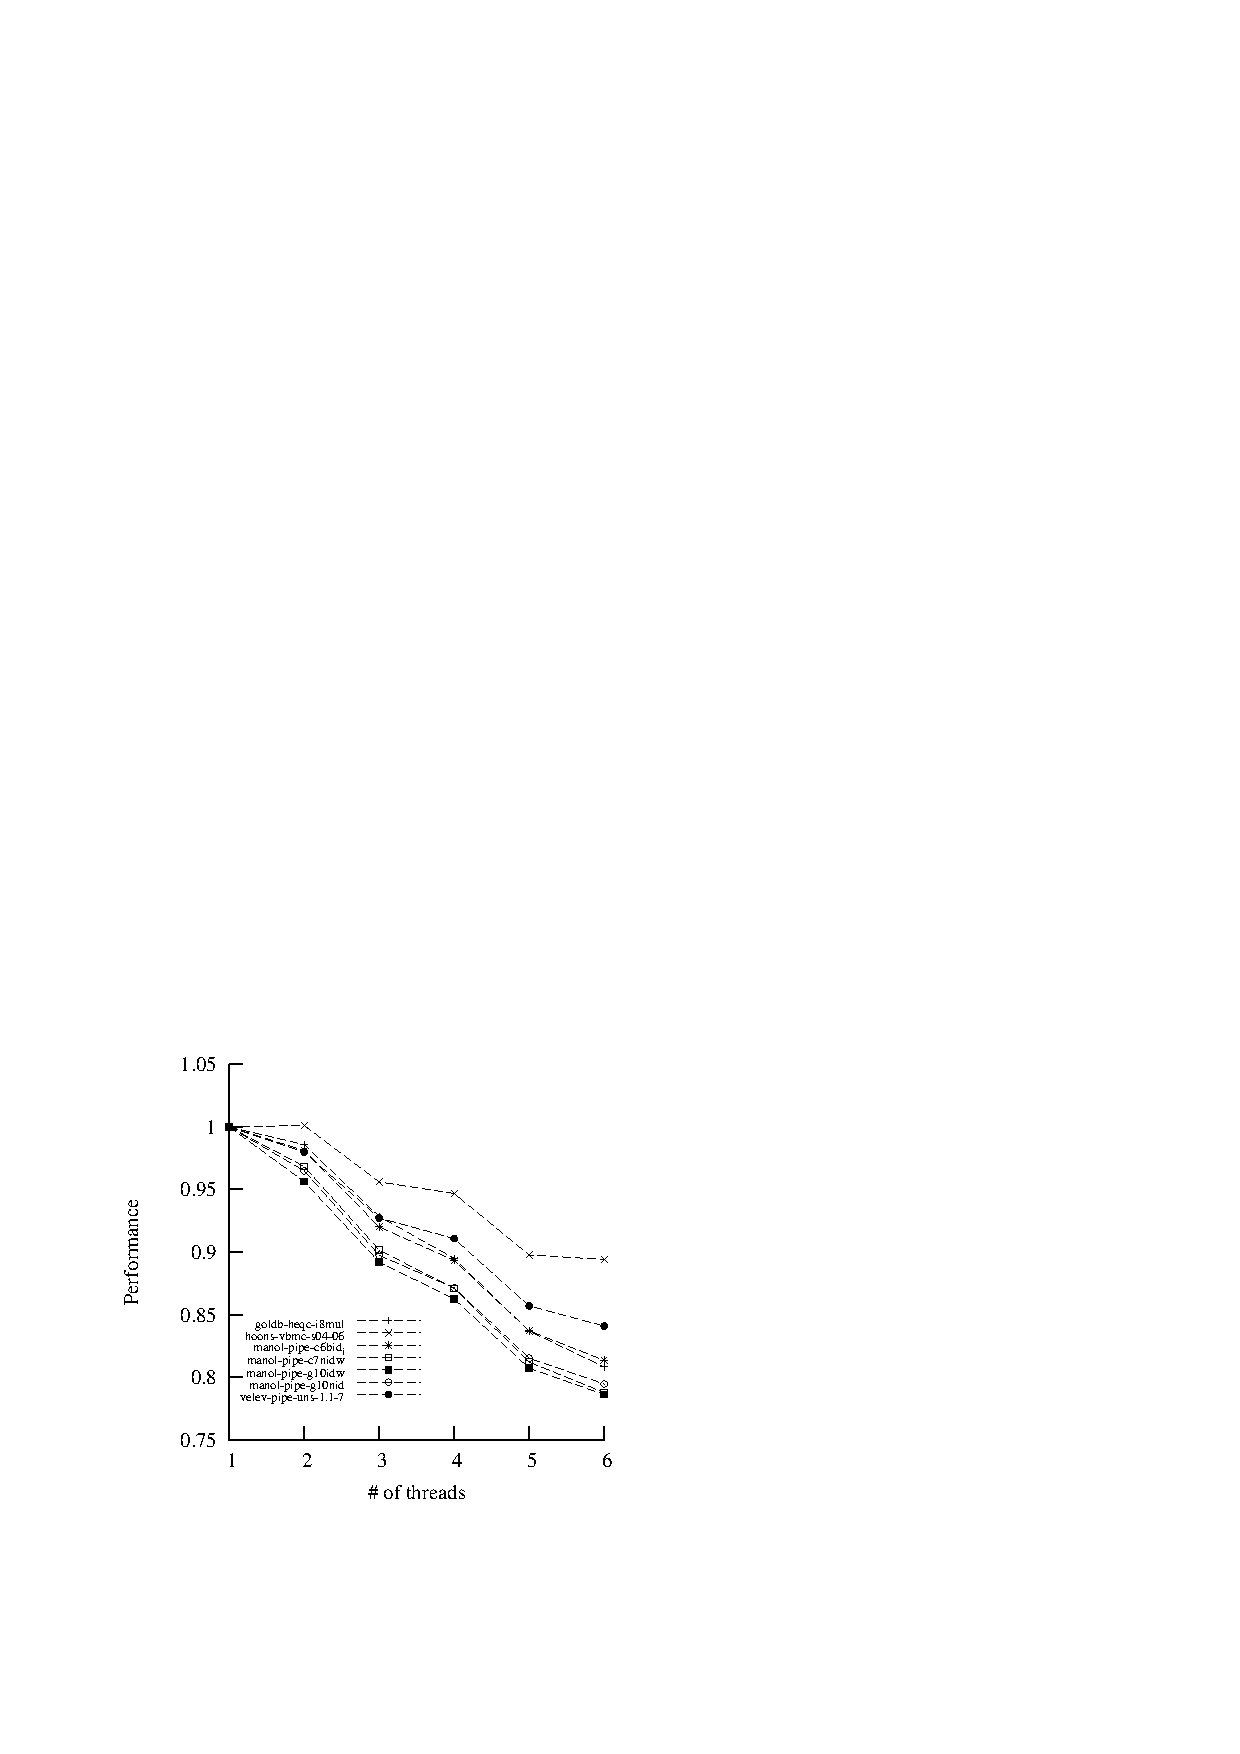
\includegraphics[scale=1]{plingeling_6cores_speedup}
  \caption{Performance decay of {\tt plingeling} when run over many cores}
  \label{fig:decay}
\end{figure}

In order to find the culprit of the performance decay, we have
developed a simple portfolio-based SAT solver that allows us to
replicate the behavior of \pling, and then also experiment with
alternative scenarios in order to take measures towards the
improvement of its performance.

% Solvers implementando el portfolio-approach. Realizando experimentos,
% hemos notado que varios cdcl SAT-solvers ejecutándose en un mismo
% procesador (de varios cores) tienden a decaer en rendimiento
% individual (aprox 8 por core usado) en comparación a ejecuciones en
% procesadores distintos o de forma solitaria (Experimentos con
% Barcelogic en el cluster de máquinas). Este fenómeno (creemos, debido
% a que comparten Cache) se observa también en Portfolio-approach-based
% SAT-solvers que no comparten memoria (experimentos con Plingeling). El
% estudio que realizamos es ver si lo mismo ocurre en
% Portfolio-approach-based SAT-solvers que SI comparten memoria (al
% estilo SArTagnan, ahora que lo conocemos, e inspirados en el modelo de
% miraXT). Para ello, hemos implementado un portfolio-approach-based
% SAT-solver muy sencillo, modificado de tal manera que nos deje
% realizar experimentos al respecto y, de ser posible, tomar algunas
% medidas de la ejecución (habría que ver si el perf nos da algo en qué
% apoyarnos). Lo ideal sería replicar la búsqueda (distinta en todos los
% casos) de varios hilos cdcl con memoria independiente, en un modelo de
% memoria distribuida, pero, como esto es muy difícil de hacer sin
% sabotear bastante el rendimiento de los solvers de memoria compartida
% (al menos, no se me ocurre muy bien cómo hacerlo), nosotros realizamos
% el experimento con búsquedas idénticas en todos los hilos (cosa que se
% puede implementar en memoria compartida sin perjudicar mucho su
% rendimiento). Hasta que no tengamos nuestro solver, no sabemos qué
% conclusión tenemos. Según experimentos con matrices de Juan, la cosa
% no está tan clara, esperemos que la cosa vaya bien.

\section{The AzuDICI SAT Solver}
\label{sec:azudici}




% We recommend abbrvnat bibliography style.
\bibliographystyle{splncs}

% The bibliography should be embedded for final submission.
\bibliography{sat}

\end{document}
